% --- LaTeX Presentation Template - S. Venkatraman ---

% --- Set document class ---

% Remove "handout" when presenting to include pauses
\documentclass[dvipsnames, handout]{beamer}
\usepackage{layout}
\usepackage{caption}
\usepackage{subcaption}
\usetheme{default}
\usepackage{textcomp}
\usepackage{pifont}
\usepackage{subcaption}
\usepackage{tabularx}
\usepackage[inline]{asymptote}


% Make content that is hidden by pauses "transparent"
\setbeamercovered{transparent}

% --- Slide layout settings ---

% Set line spacing
\renewcommand{\baselinestretch}{1.15}

% Set left and right text margins
\setbeamersize{text margin left=8mm, text margin right=8mm}


% Add slide numbers in bottom right corner
\setbeamertemplate{footline}[frame number]

% Remove navigation symbols
\setbeamertemplate{navigation symbols}{}

% Allow local line spacing changes
\usepackage{setspace}

% --- Color and font settings ---
% We will mainly use 2 colors: uofsc-red-primary, black
% We will use several font sizes to differentiate title, subtitle, normal text, etc.

\usepackage{xcolor}

% define theme colors
\definecolor{uofsc-red-primary}{HTML}{73000a}
\definecolor{uofsc-red-rose}{HTML}{cc2e40}
\definecolor{uofsc-red-dark}{HTML}{570008}

% Change itemized list bullets to circles
\setbeamertemplate{itemize item}{\color{uofsc-red-rose}$\bullet$}
\setbeamertemplate{itemize subitem}{\color{uofsc-red-rose}$\circ$}

\setbeamertemplate{enumerate item}{\color{uofsc-red-rose}\arabic{enumi}.}

% Slide title background color
\definecolor{background}{HTML}{ffffff}

% Slide title text color
\definecolor{titleText}{HTML}{73000a}

% Other possible color schemes

% - Light green/dark green -
%\definecolor{background}{HTML}{e4ede4}
%\definecolor{titleText}{HTML}{2e592f}

% - Light blue/dark blue -
%\definecolor{background}{HTML}{d5d9e8}
%\definecolor{titleText}{HTML}{2d375e}

% - Beige/dark blue -
%\definecolor{background}{HTML}{e8e2d5}
%\definecolor{titleText}{HTML}{2d3375}

% Set colors
\setbeamercolor{frametitle}{bg=background, fg=titleText}
\setbeamercolor{title}{fg=uofsc-red-primary}
\setbeamercolor{subtitle}{fg=uofsc-red-primary}

% Set font sizes for frame title and subtitle
\setbeamerfont{frametitle}{size=\fontsize{15}{16}}
\setbeamerfont{framesubtitle}{size=\small}

% --- Math/Statistics commands ---

% Add a reference number to a single line of a multi-line equation
% Usage: "\numberthis\label{labelNameHere}" in an align or gather environment
\newcommand\numberthis{\addtocounter{equation}{1}\tag{\theequation}}

% Shortcut for bold text in math mode, e.g. $\b{X}$
\let\b\mathbf

% Shortcut for bold Greek letters, e.g. $\bg{\beta}$
\let\bg\boldsymbol

% Shortcut for calligraphic script, e.g. %\mc{M}$
\let\mc\mathcal

% \mathscr{(letter here)} is sometimes used to denote vector spaces
\usepackage[mathscr]{euscript}

% Convergence: right arrow with optional text on top
% E.g. $\converge[p]$ for converges in probability
\newcommand{\converge}[1][]{\xrightarrow{#1}}

% Weak convergence: harpoon symbol with optional text on top
% E.g. $\wconverge[n\to\infty]$
\newcommand{\wconverge}[1][]{\stackrel{#1}{\rightharpoonup}}

% Equality: equals sign with optional text on top
% E.g. $X \equals[d] Y$ for equality in distribution
\newcommand{\equals}[1][]{\stackrel{\smash{#1}}{=}}

% Normal distribution: arguments are the mean and variance
% E.g. $\normal{\mu}{\sigma}$
\newcommand{\normal}[2]{\mathcal{N}\left(#1,#2\right)}

% Uniform distribution: arguments are the left and right endpoints
% E.g. $\unif{0}{1}$
\newcommand{\unif}[2]{\text{Uniform}(#1,#2)}

% Independent and identically distributed random variables
% E.g. $ X_1,...,X_n \iid \normal{0}{1}$
\newcommand{\iid}{\stackrel{\smash{\text{iid}}}{\sim}}

% Sequences (this shortcut is mostly to reduce finger strain for small hands)
% E.g. to write $\{A_n\}_{n\geq 1}$, do $\bk{A_n}{n\geq 1}$
\newcommand{\bk}[2]{\{#1\}_{#2}}

% Math mode symbols for common sets and spaces. Example usage: $\R$
\newcommand{\R}{\mathbb{R}}	% Real numbers
\newcommand{\C}{\mathbb{C}}	% Complex numbers
\newcommand{\Q}{\mathbb{Q}}	% Rational numbers
\newcommand{\Z}{\mathbb{Z}}	% Integers
\newcommand{\N}{\mathbb{N}}	% Natural numbers
\newcommand{\F}{\mathcal{F}}	% Calligraphic F for a sigma algebra
\newcommand{\El}{\mathcal{L}}	% Calligraphic L, e.g. for L^p spaces

% Math mode symbols for probability
\newcommand{\pr}{\mathbb{P}}	% Probability measure
\newcommand{\E}{\mathbb{E}}	% Expectation, e.g. $\E(X)$
\newcommand{\var}{\text{Var}}	% Variance, e.g. $\var(X)$
\newcommand{\cov}{\text{Cov}}	% Covariance, e.g. $\cov(X,Y)$
\newcommand{\corr}{\text{Corr}}	% Correlation, e.g. $\corr(X,Y)$
\newcommand{\B}{\mathcal{B}}	% Borel sigma-algebra

% Other miscellaneous symbols
\newcommand{\tth}{\text{th}}	% Non-italicized 'th', e.g. $n^\tth$
\newcommand{\Oh}{\mathcal{O}}	% Big-O notation, e.g. $\O(n)$
\newcommand{\1}{\mathds{1}}	% Indicator function, e.g. $\1_A$

% Additional commands for math mode
\DeclareMathOperator*{\argmax}{argmax}	% Argmax, e.g. $\argmax_{x\in[0,1]} f(x)$
\DeclareMathOperator*{\argmin}{argmin}	% Argmin, e.g. $\argmin_{x\in[0,1]} f(x)$
\DeclareMathOperator*{\spann}{Span}	% Span, e.g. $\spann\{X_1,...,X_n\}$
\DeclareMathOperator*{\bias}{Bias}	% Bias, e.g. $\bias(\hat\theta)$
\DeclareMathOperator*{\ran}{ran}		% Range of an operator, e.g. $\ran(T) 
\DeclareMathOperator*{\dv}{d\!}		% Non-italicized 'with respect to', e.g. $\int f(x) \dv x$
\DeclareMathOperator*{\diag}{diag}	% Diagonal of a matrix, e.g. $\diag(M)$
\DeclareMathOperator*{\trace}{trace}	% Trace of a matrix, e.g. $\trace(M)$
\DeclareMathOperator*{\supp}{supp}	% Support of a function, e.g., $\supp(f)$

% --- Presentation begins here ---

\begin{document}

% --- Title slide ---
% We have to specify the location of title, subtitle, author, dates, institutes, etc
% Right now we just put everything on the slides, without specifying the space between rows or the height of blocks.
% We will fix these details later.
% In general, we don't want to have too many different font sizes to mess up a page. The names, dates, affiliations (institutes, emails) should be of the same font size, except for some extreme cases (for example, the affiliation is too long and it has to be shrank to be fitted into the page).
% The space between title (including subtitle) to author to affiliation should keep constant. It's not the absolute location but the space in between that determines the overall look of the page.
% We will design this better, with reference to https://www.overleaf.com/learn/latex/Beamer


\title{FAB-MAP: Probabilistic Localization and Mapping in the Space of Appearance}
%\subtitle{Progress Report}
\author{Presented by\\ Zifei (David) Zhong\vspace{-.3cm}}

%\institute{Dept. of Computer Science and Engineering, \\Dept. of Exercise Science, \\University of South Carolina}
\date{11/13/2023}
\begin{frame}
\titlepage
\vspace{1.2cm}

\begin{center}
%\include-graphics[width=1cm]{imgs/uofsc-logo.png}\bigskip
{\begin{spacing}{1.2}\scriptsize 
authored by Mark Cummins and Paul Newman;\\
appeared in the International Journal of Robotics Research, 2008
\end{spacing}}
\end{center}
\end{frame}

% --- Main content ---

% Example slide: use \pause to sequentially unveil content


\begin{frame}[t]{Introducation}
\framesubtitle{Fast Appearance-Based Mapping (FAB-MAP)}

\begin{itemize}
\item Problem: Recognizing locations based on their appearance.
\item Solution: Learning a generative model for the appearance to achieve:
\begin{enumerate}
\item Compute the similarity of two observations.
\item Compute the probability that the two observations originate from the same location.
\end{enumerate}
\item Superiorities: 
\begin{enumerate}
\item Address perceptual aliasing (less false positives)
\item Improve inference reasoning (less false negatives)
\item Accommodate new locations
\item Linear-time complexity
\end{enumerate}
\end{itemize}

\end{frame}


\begin{frame}[t]{Chow Liu Tree}
\framesubtitle{Approximating High Dimensional Discrete Distributions}
\begin{itemize}
\item The Chow Liu algorithm approximates a discrete distribution $P(Z)$ by the closest tree-structured Bayesian network $Q(Z)_{opt}$, in the sense of minimizing the Kullback-Leibler divergence.
\item For a distribution over $n$ variables, a mutual information graph $\mathcal{G}$ is the complete graph with $n$ nodes and $\frac{n(n-1)}{2}$ edges, where each edge $(z_i, z_j)$ has weight equal to the mutual information $I(z_i, z_j)$ between variable $i$ and $j$: 
\[I(z_i, z_j) = \sum_{z_i \in \Omega, z_j \in \Omega} p(z_i, z_j) \log \frac{p(z_i, z_j)}{p(z_i)p(z_j)}\]

\end{itemize}
\end{frame}

\begin{frame}[t]{Chow Liu Tree}
\framesubtitle{Advantages \& Illustration}
\begin{itemize}
\item The maximum-weight spanning tree of the mutual information graph $\mathcal{G}$ will have the same structure as $Q(Z)_{opt}$.
\item The Chow Liu algorithm guarantees the optimal approximation, and requires only first order conditional probabilities.
\end{itemize}

\begin{center}
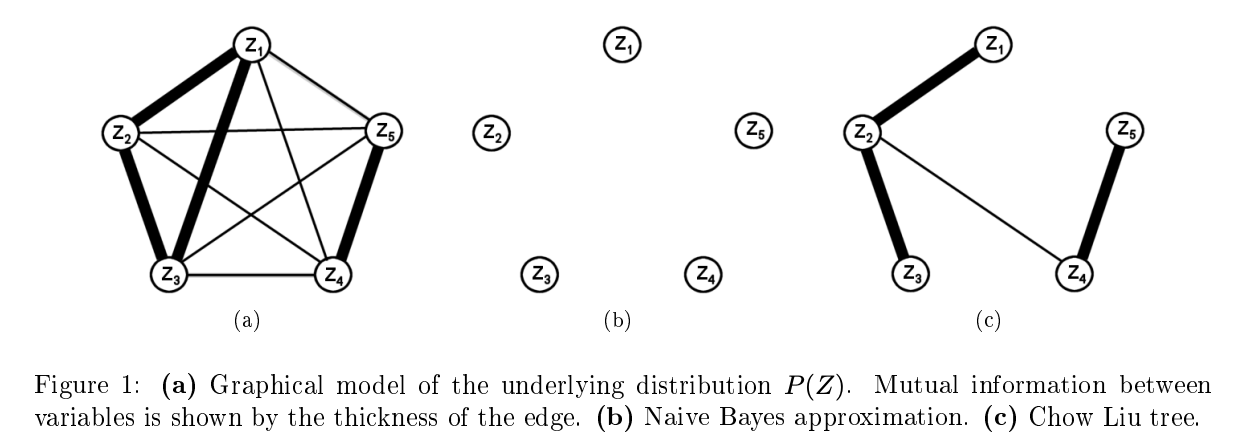
\includegraphics[width=0.75\textwidth]{imgs/fig1.png}
\end{center}
\end{frame}

\begin{frame}[t]{Probabilistic Navigation using Appearance}
\framesubtitle{Overview}
\begin{itemize}
\item The world is modeled as a set of discrete locations, each location being described by a distribution over ``appearance words''.
\item Incoming sensory data is converted into a bag-of-words representation.
\item For each location $L_i$, we ask how likely it is that the observation comes from $L_i$'s distribution.
\item Find the probability that the observation comes from a location not in the map, and update the map if a location found.
\end{itemize}
\end{frame}


\begin{frame}[t]{Probabilistic Navigation using Appearance}
\framesubtitle{Representing Appearance}
\begin{itemize}
\item ``bag-of-words'' representation for raw sensor data
\begin{enumerate}
\item A scene is represented as a collection of attributes (words) chosen from a set (vocabulary) of size $|v|$.
\end{enumerate}
\item Observation $Z_k$ of local scene appearance at time $k$:
\begin{enumerate}
\item $Z_k = \{z_1, \cdots, z_{|v|} \}$
\item $z_i$ is a binary variable indicating the presence/absence of the $i$th word of the vocabulary.
\end{enumerate}

\end{itemize}
\end{frame}



\begin{frame}[t]{Probabilistic Navigation using Appearance}
\framesubtitle{Representing Locations}
\begin{itemize}
\item Map of environment at time $k$ is a collection of $n_k$ discrete and disjoint locations $\mathcal{L}^k = \{L_1, \cdots, L_{n_k}\}$.
\item Hidden variable $e_i$: an event that an object which generates observations of type $z_i$ exists.
\item Location $L_i$'s model: a set $\{p(e_1=1|L_i), \cdots, p(e_{|v|}=1|L_i)\}$, where each $e_i$ is generated independently by the location.
\item Detector $\mathcal{D}$:
\[\mathcal{D}: 
\begin{cases} 
p(z_i=1|e_i=0) , \text{false positive probability}\\
p(z_i=0|e_i=1) , \text{false negative probability}
\end{cases}    \]
\end{itemize}
\end{frame}


\begin{frame}[t]{Probabilistic Navigation using Appearance}
\framesubtitle{Representing Locations: illustration}
\begin{itemize}
\item Factoring $p(Z|L_i)$ into two parts:
\begin{enumerate}
\item (Learn online) A simple model that $e_i$ only depends on $L_i$.
\item (Learn offline) A complex model that captures the correlations between detections of appearance words $p(z_i|Z_k)$.
\end{enumerate}
\end{itemize}
\begin{center}
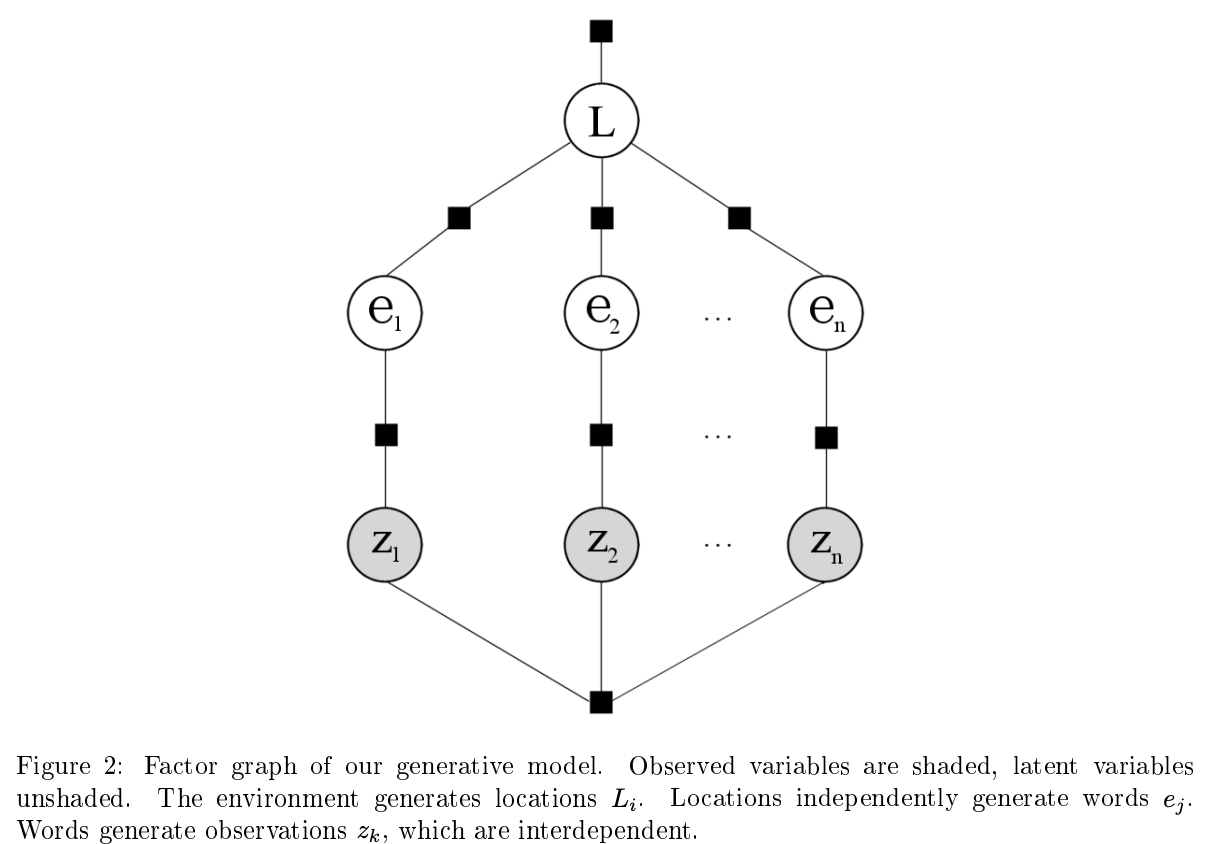
\includegraphics[width=0.55\textwidth]{imgs/fig2.png}
\end{center}
\end{frame}

\begin{frame}[t]{Probabilistic Navigation using Appearance}
\framesubtitle{Estimating Location via Recursive Bayes}
\begin{itemize}
\item Calculating $p(L_i|\mathcal{Z}^k)$:
\[p(L_i|\mathcal{Z}^k) = \frac{p(Z_k|L_i, \mathcal{Z}^{k-1})p(L_i|\mathcal{Z}^{k-1})}{p(Z_k|\mathcal{Z}^{k-1})}\]
\begin{enumerate}
\item $\mathcal{Z}^k$: the set of all observations up to time $k$
\item $p(L_i|\mathcal{Z}^{k-1})$: prior belief about our location
\item $p(Z_k|L_i, \mathcal{Z}^{k-1})$: observation likelihood, equal to $p(Z_k|L_i)$
\item $p(Z_k|\mathcal{Z}^{k-1})$: normalization term
\end{enumerate}
\end{itemize}
\end{frame}

\begin{frame}[t]{Probabilistic Navigation using Appearance}
\framesubtitle{Observation Likelihood}
\begin{itemize}
\item Naive Bayes assumption: 
\[p(Z_k|L_i) \approx p(z_n|L_i)\cdots p(z_2|L_i)p(z_1|L_i),\]
and 
\begin{align*}
p(z_j|L_i) &= \sum_{s\in\{0,1\}} p(z_j|e_j=s, L_i)p(e_j=s|Li)\\
& =  \sum_{s\in\{0,1\}} p(z_j|e_j=s)p(e_j=s|Li)
\end{align*}
\end{itemize}
\end{frame}

\begin{frame}[t]{Probabilistic Navigation using Appearance}
\framesubtitle{Observation Likelihood}
\begin{itemize}
\item Chow Liu assumption: 
\[p(Z_k|L_i) \approx p(z_r|L_i)\prod_{q=2}^{|v|} p(z_q|z_{p_q},L_i),\]
where $z_r$ is the root of the tree, and $z_{p_q}$ is the parent of $z_q$ in the tree. With further expansion,
\[p(z_q|z_{p_q, L_i})  = \sum_{s_{e_a} \in \{0,1\}} p(z_q|e_q=s_{e_q}, z_{p_q})p(e_q=s_{e_q}|L_i),\]
\[p(z_q|e_q,z_{p_q}) \approx \left(1+\frac{\alpha}{\beta}\right)^{-1},\]

\end{itemize}
\end{frame}

\begin{frame}[t]{Probabilistic Navigation using Appearance}
\framesubtitle{Observation Likelihood}
where 
\[\alpha = p(z_q=s_{z_q})p(z_q=\bar{s_{z_q}}|e_q=s_{e_q})p(z_q=\bar{s_{z_q}}|z_p=s_{z_p}),\]
\[\beta = p(z_q=\bar{s_{z_q}})p(z_q=s_{z_q}|e_q=s_{e_q})p(z_q=s_{z_q}|z_p=s_{z_p}),\]

Now, $\alpha$ and $\beta$ are expressed entirely in terms of quantities that can be estimated from training data. 
\end{frame}


\begin{frame}[t]{Probabilistic Navigation using Appearance}
\framesubtitle{Discovery of New Places}
\begin{itemize}
\item To deal with the possibility that a new observation comes from a previously unknown location, calculation of $p(Z_k|\mathcal{Z}^{k-1})$ is required.
\item Dividing the world into two sets: mapped places $M$, and unmapped places $\bar{M}$, then
\begin{align*}
p(Z_k|\mathcal{Z}^{k-1}) &\approx \sum_{m\in M} p(Z_k|L_m)p(L_m|\mathcal{Z}^{k-1})\\ 
&+ p(L_{new}|\mathcal{Z}^{k-1})\sum_{u=1}^{n_s}\frac{p(Z_k|L_u)}{n_s}
\end{align*}
where $n_s$ is the number of samples, and $p(L_{new}|\mathcal{Z}^{k-1})$ is the prior probability of being at a new place.
\end{itemize}
\end{frame}


\begin{frame}[t]{Probabilistic Navigation using Appearance}
\framesubtitle{Location Prior \& Smoothing}
\begin{itemize}
\item With sequentially collected observations, if the robot is at place $i$ at time $t$, it has equal probability of being at one of the places $\{i-1, i, i+1\}$ at time $t+1$; otherwise assume uniform prior.
\item Smoothing the likelihood estimation:
\[p(Z_k|L_i) \rightarrow \sigma p(Z_k|L_i) + \frac{1-\sigma}{n_k}, \]
where $n_k$ is the number of places in the map, $\sigma$ is the smoothing parameter (0.99 in experiments).
\end{itemize}
\end{frame}


\begin{frame}[t]{Probabilistic Navigation using Appearance}
\framesubtitle{Updating Place Models}
\begin{itemize}
\item When a new place is created, its appearance model is initialized so that all words exist with marginal probability $p(e_i=1)$ derived from the training data.
\item Given an observation that relates to the new place, each component of the appearance model can be updated by
\[p(e_i=1|L_j,\mathcal{Z}^k) = \frac{p(Z_k|e_i=1,L_j)p(e_i=1|L_j, \mathcal{Z}^{k-1})}{p(Z_k|Lj)}\]
\end{itemize}

\end{frame}


\begin{frame}[t]{Probabilistic Navigation using Appearance}
\framesubtitle{Input Parameters}
\begin{itemize}
\item Detector model, $p(z_i=1|e_i=0)$ and $p(z_i=0|e_i=1)$.
\item Smoothing parameter $\sigma$.
\item Prior probability that a topological link with an unknown endpoint leads to a new place.
\end{itemize}

\end{frame}

\begin{frame}[t]{Evaluation}
\framesubtitle{Building the Vocabulary Model}
\begin{itemize}
\item Use the SURF detector/description to extract region of interest from images, and map the 128D descriptors  visual words.
\item Construct Chow Liu tree.
\begin{enumerate}
\item Each node in the graph corresponds to a visual word.
\item Compute the maximum-weight spanning tree of the graph.
\item 2800 images from 28km of urban streets environment.
\item 11k visual words in the constructed Chow Liu tree.
\end{enumerate}
\end{itemize}

\end{frame}

\begin{frame}[t]{Sample Vocabulary }
\begin{center}
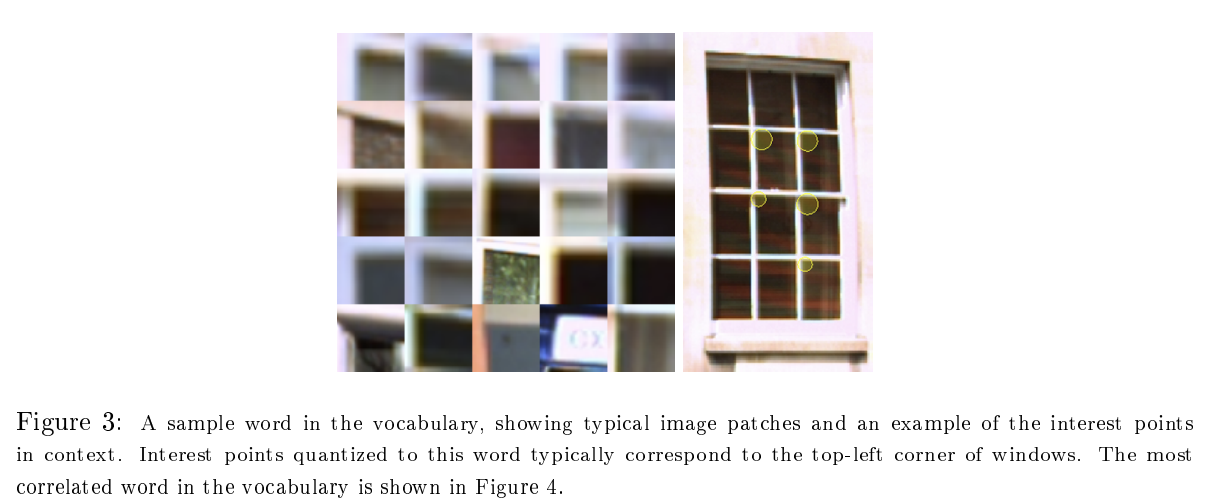
\includegraphics[width=0.75\textwidth]{imgs/fig3.png}
\end{center}
\begin{center}
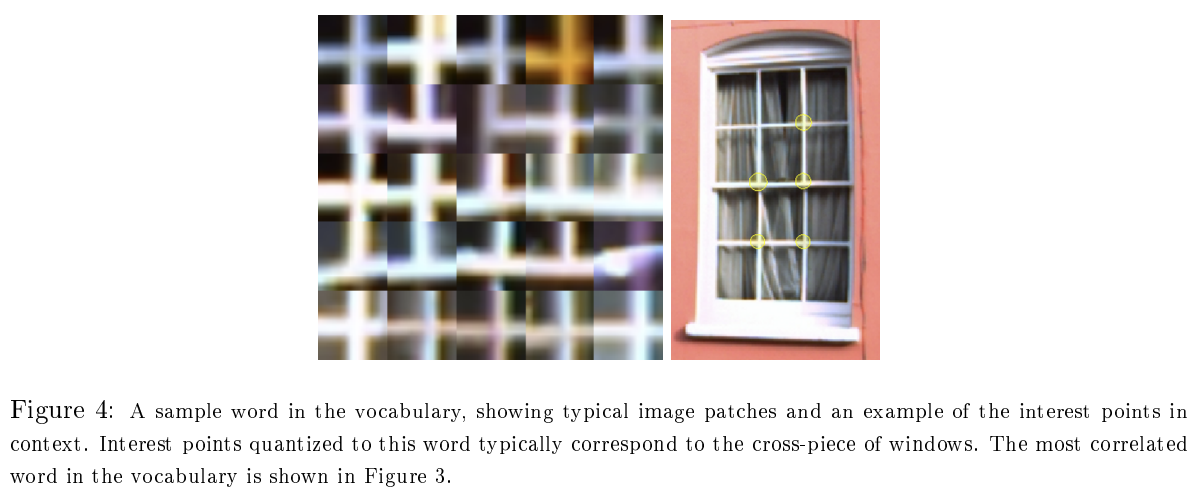
\includegraphics[width=0.75\textwidth]{imgs/fig4.png}
\end{center}
\end{frame}

\begin{frame}[t]{Sample Chow Liu Tree}
\begin{center}
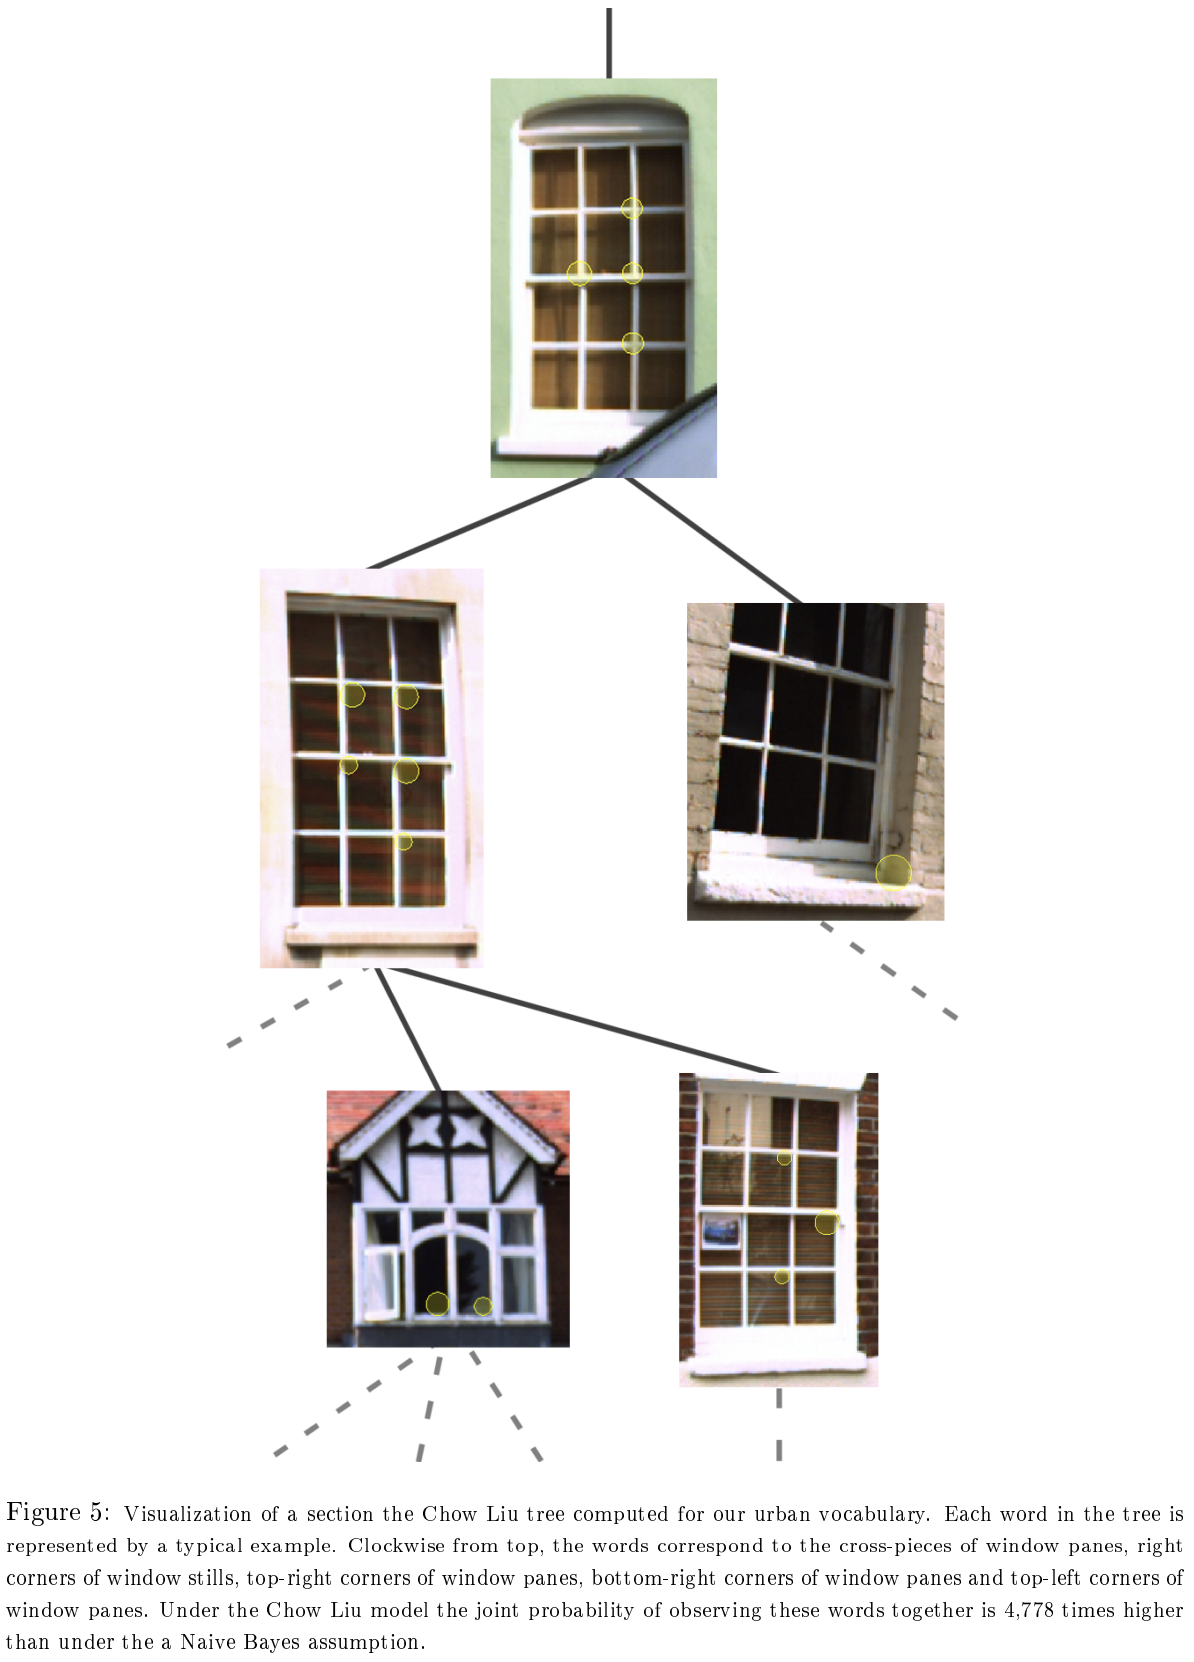
\includegraphics[width=0.5\textwidth]{imgs/fig5.png}
\end{center}
\end{frame}


\begin{frame}[t]{Appear-based Matching (City Centre dataset)}
\begin{center}
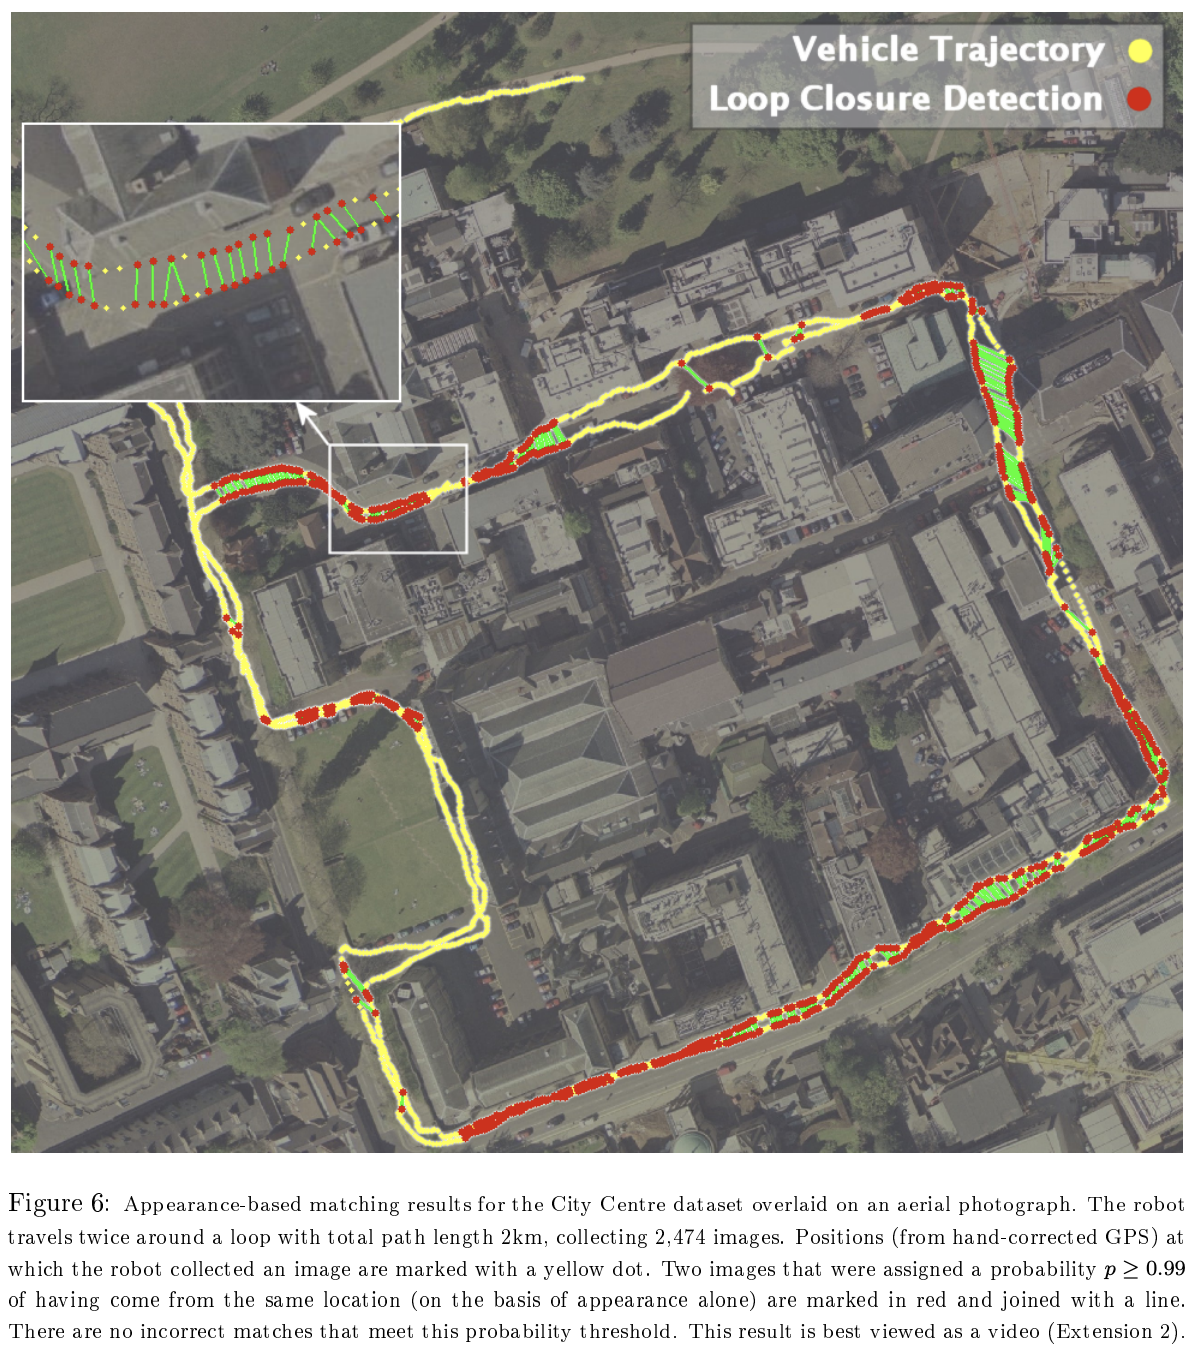
\includegraphics[width=0.6\textwidth]{imgs/fig6.png}
\end{center}
\end{frame}

\begin{frame}[t]{Appear-based Matching (New College dataset)}
\begin{center}
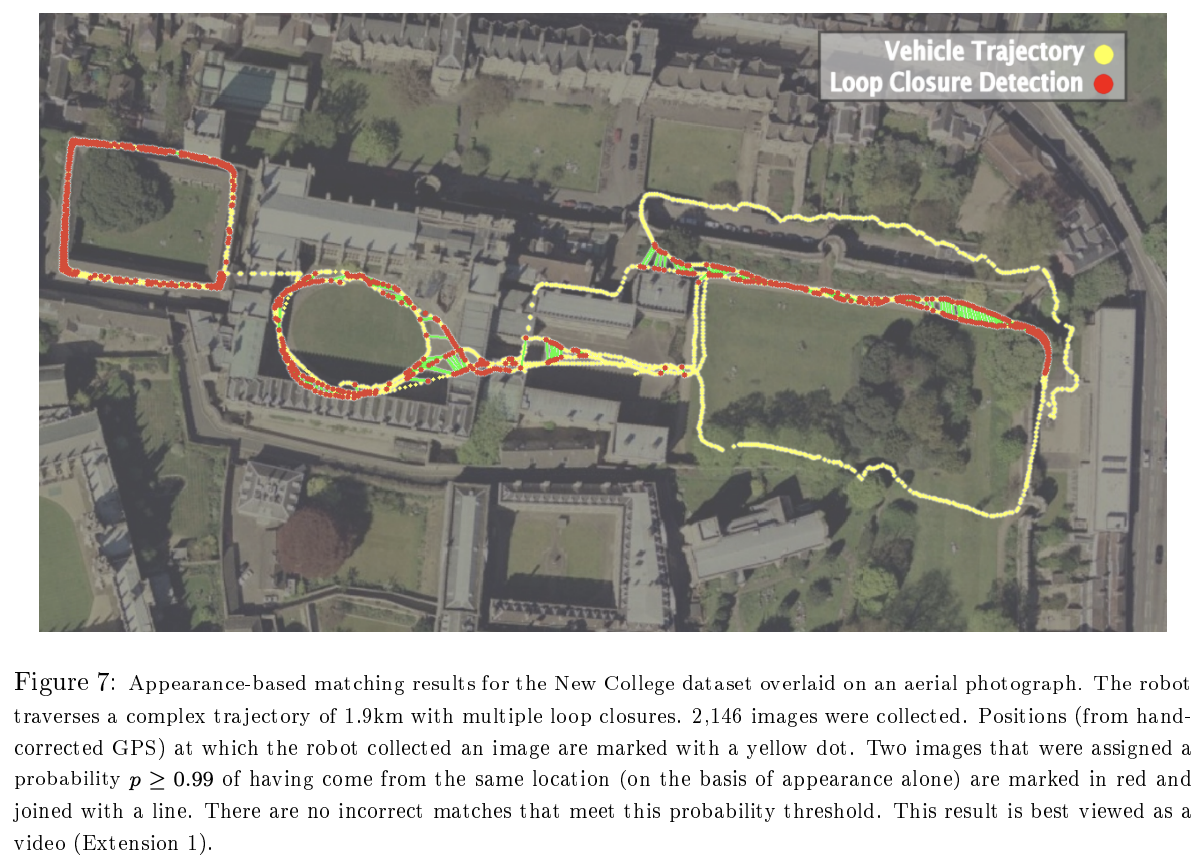
\includegraphics[width=0.75\textwidth]{imgs/fig7.png}
\end{center}
\end{frame}

\begin{frame}[t]{Precision Recall}
\begin{itemize}
\item At 100\% precision, the system achieves 48\% recall on the New College dataset, and 37\% on the City Center dataset. 
\item Typically 37\% recall rate is sufficient to detect almost all loop closure.
\end{itemize}

\begin{center}
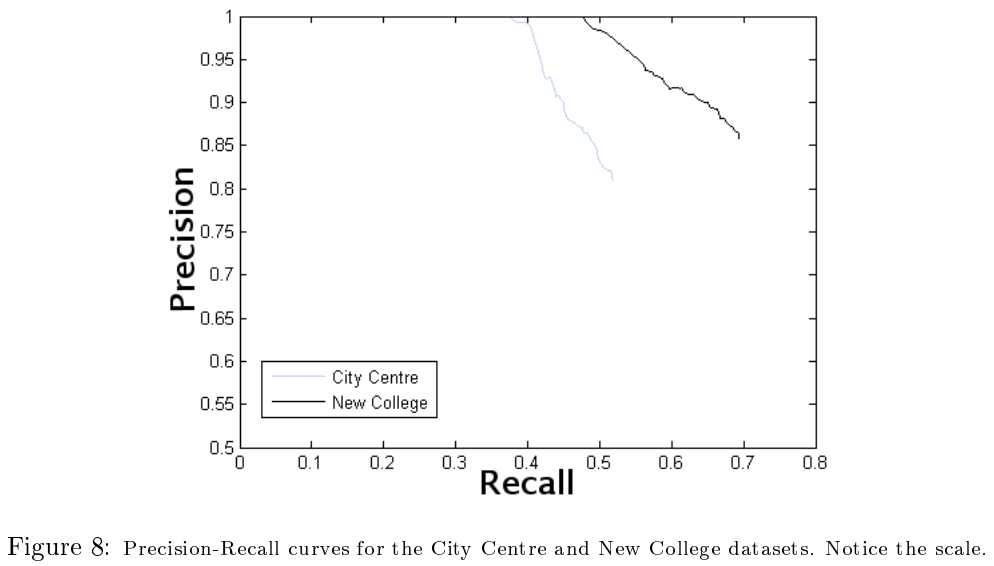
\includegraphics[width=0.75\textwidth]{imgs/fig8.png}
\end{center}
\end{frame}

\begin{frame}[t]{Samples from Results: similar scenes, different locations}
\begin{center}
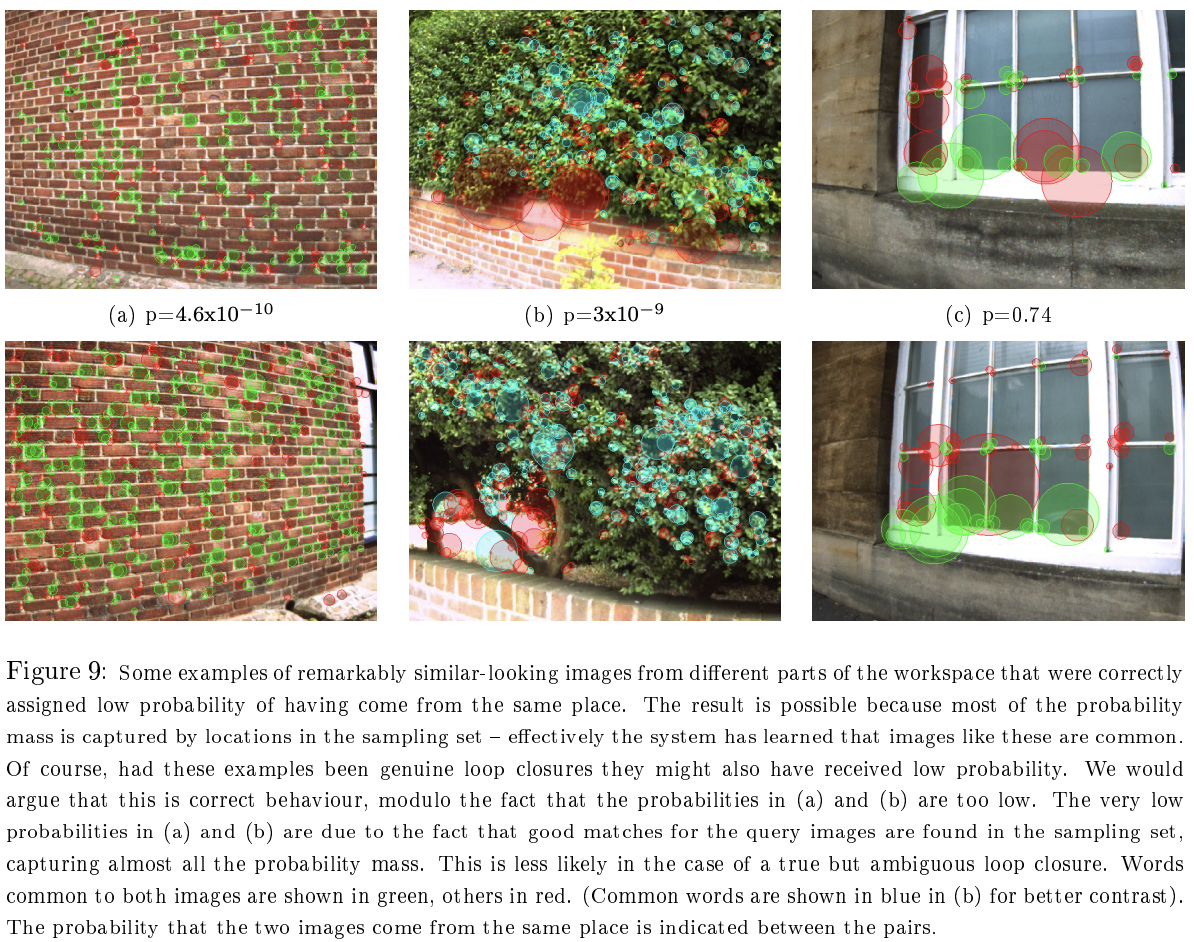
\includegraphics[width=0.75\textwidth]{imgs/fig9.png}
\end{center}
\end{frame}

\begin{frame}[t]{Samples from Results: different scenes, same location}
\begin{center}
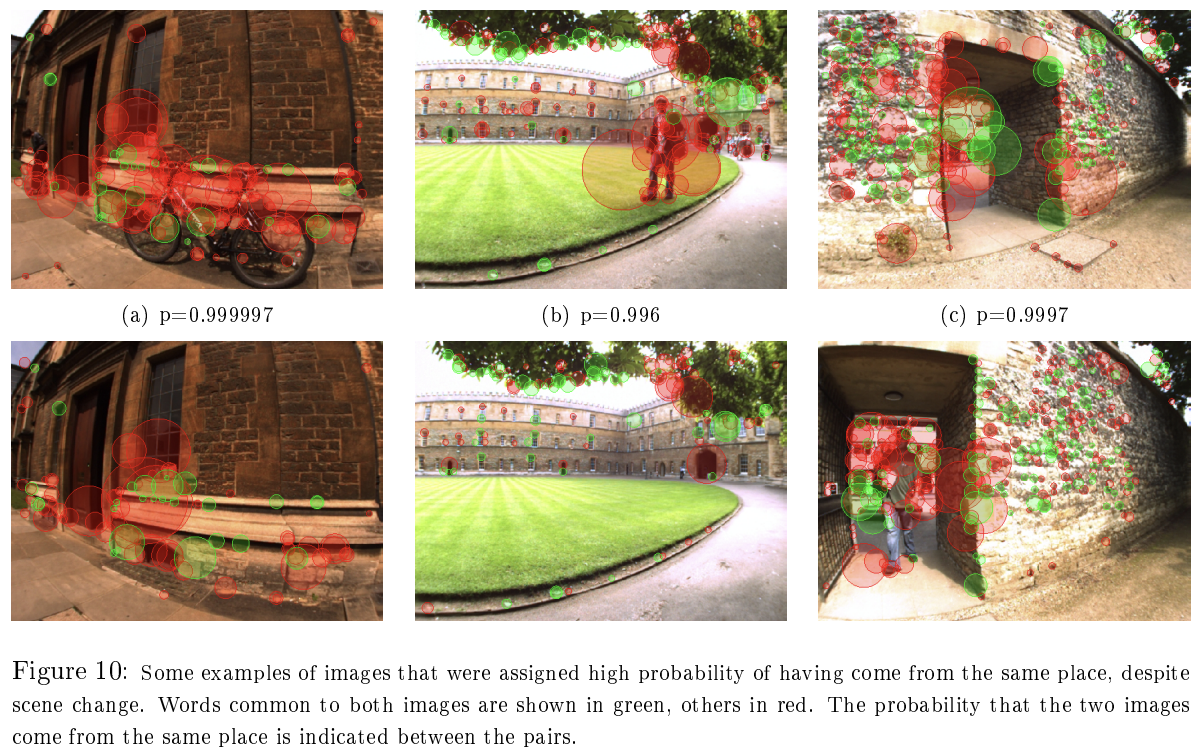
\includegraphics[width=0.75\textwidth]{imgs/fig10.png}
\end{center}
\end{frame}

\begin{frame}[t]{Comparison of Different Approximations}
\begin{center}
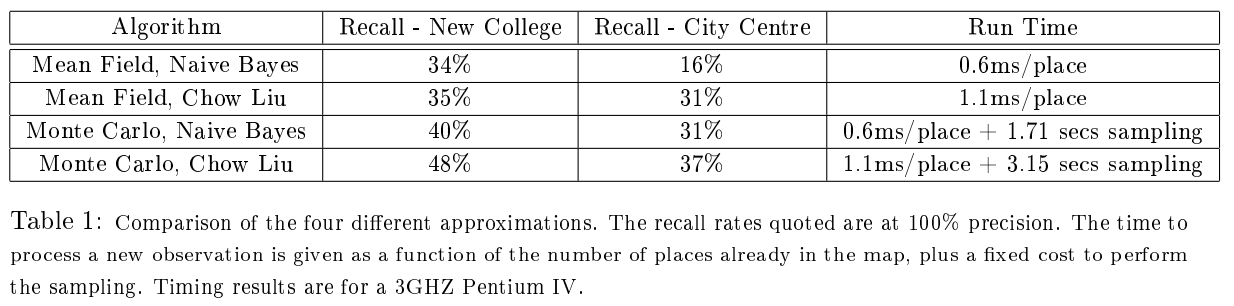
\includegraphics[width=0.75\textwidth]{imgs/table1.png}
\end{center}

\begin{center}
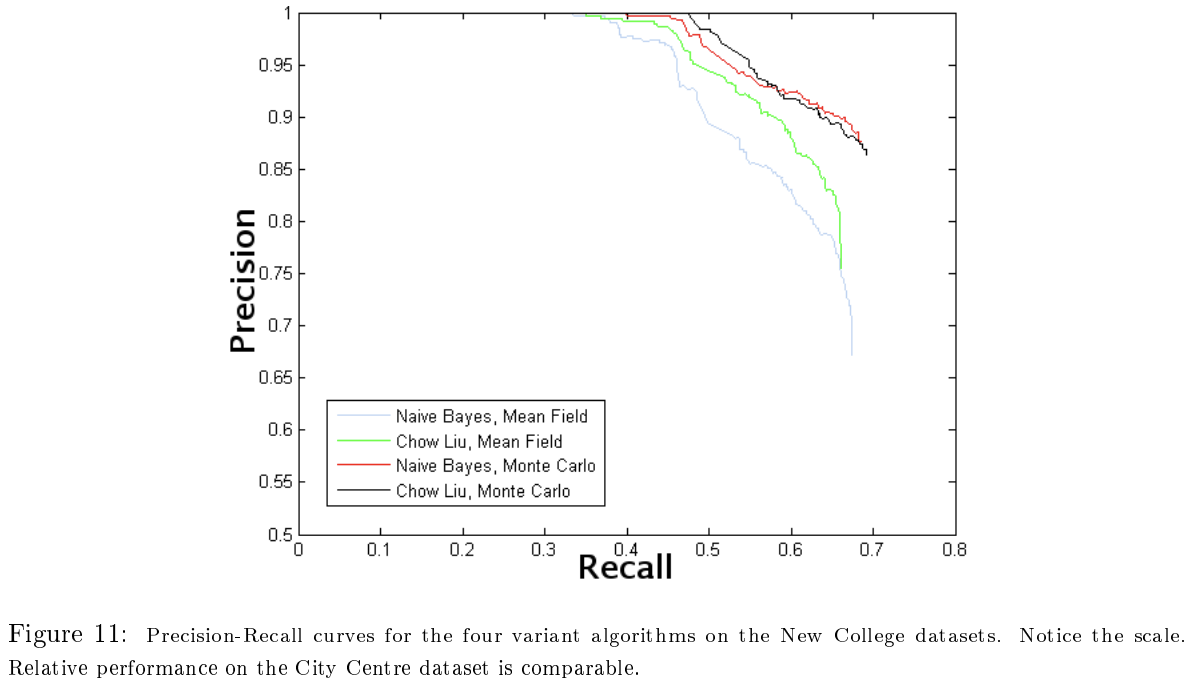
\includegraphics[width=0.75\textwidth]{imgs/fig11.png}
\end{center}
\end{frame}

\begin{frame}[t]{Chow Liu Approximation vs. Naive Bayes}
\begin{center}
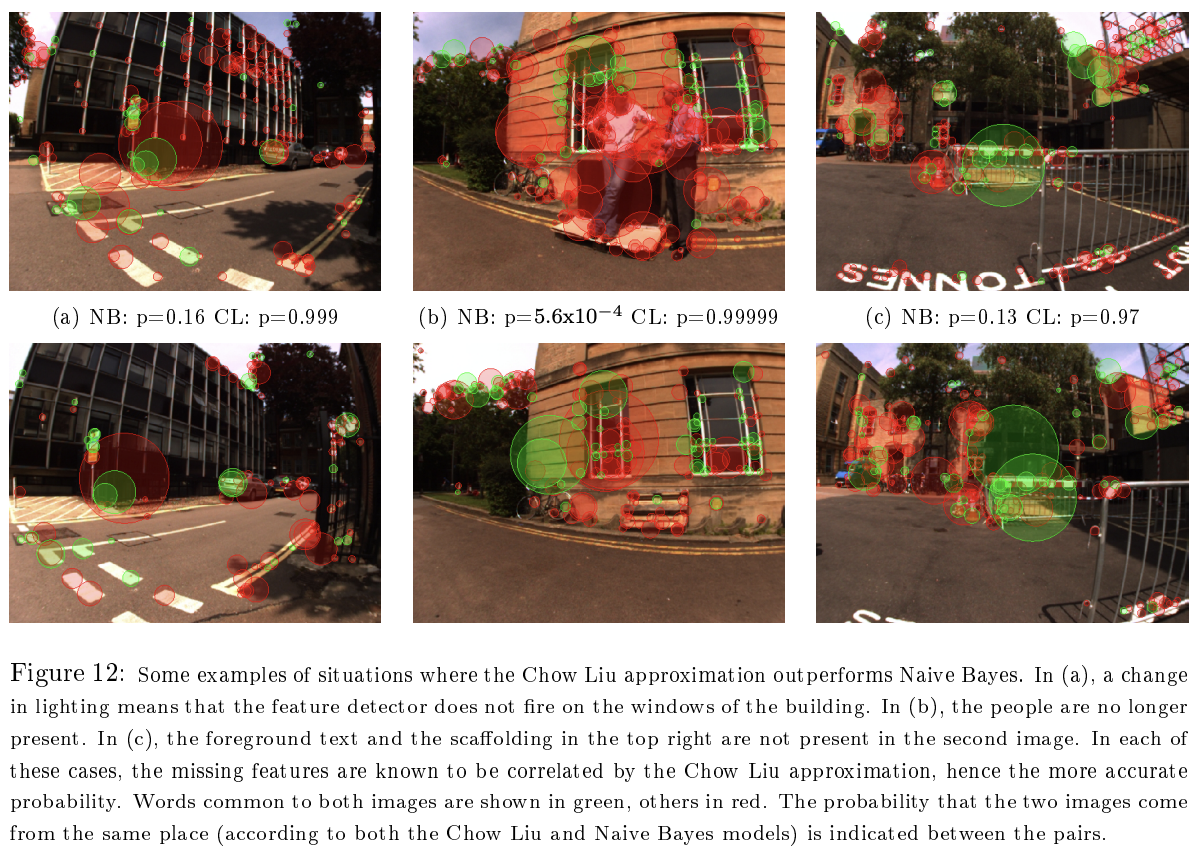
\includegraphics[width=0.75\textwidth]{imgs/fig12.png}
\end{center}
\end{frame}

\begin{frame}[t]{False Positives Possibility \& Discussion}
\begin{center}
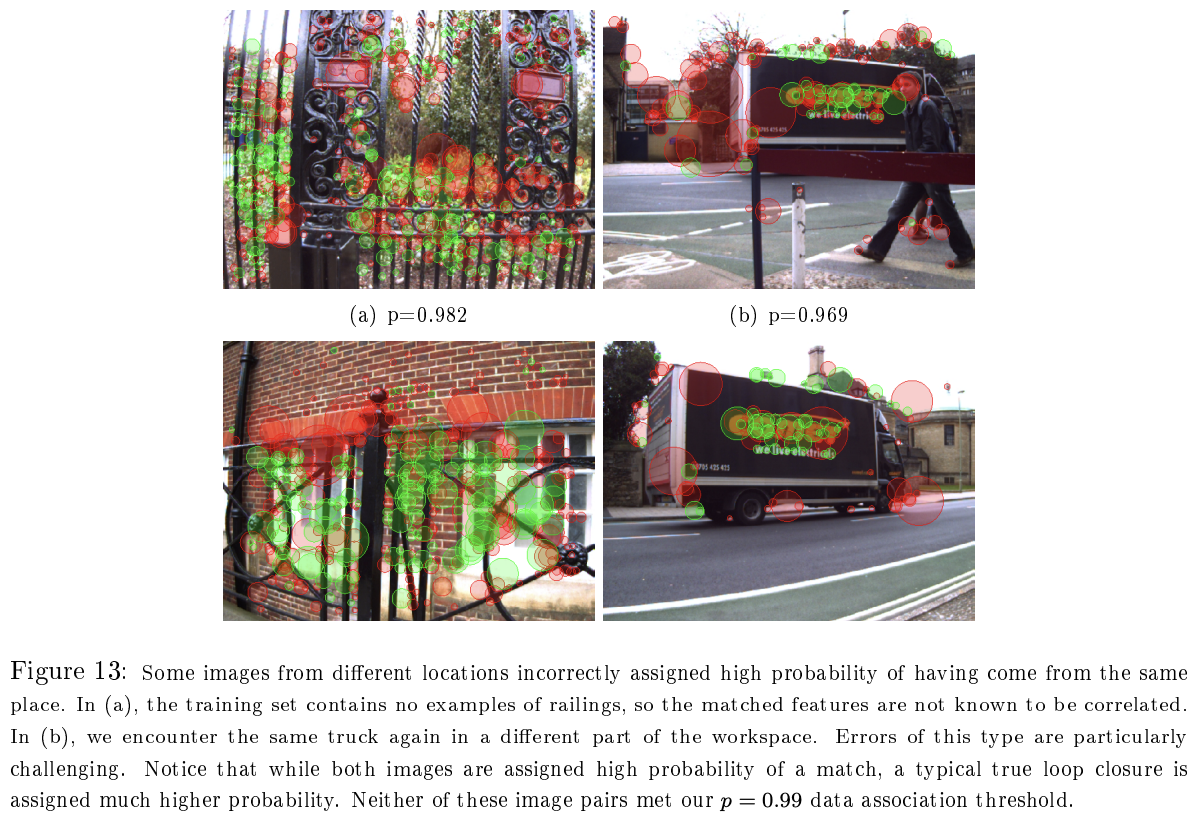
\includegraphics[width=0.75\textwidth]{imgs/fig13.png}
\end{center}
\end{frame}



\begin{frame}{References}
\begin{thebibliography}{10}
\beamertemplatearticlebibitems
{\small

\bibitem{Paper1}
Probabilistic Appearance Based Navigation and Loop Closing.
\newblock Mark  Cummins, Paul Newman. \\
{\it Proc. of IEEE International Conference on Robotics and Automation}, 2007.

\bibitem{Paper2}
Video Google: A Text Retrieval Approach to Object Matching in Videos.
\newblock Josef Sivic, Andrew Zisserman \\
{\it Proc. of IEEE International Conference on Computer Vision}, 2003.


}
\end{thebibliography}
\end{frame}










% --- Bibliography slide ---

%\begin{frame}{References}
%\begin{thebibliography}{10}
%\beamertemplatearticlebibitems
%{\small

%\bibitem{Paper1}
%Paper 1 Title.
%\newblock Paper 1 Authors. \\
%{\it Journal Name} Edition, Year.

%\bibitem{Paper 2}
%Paper 2 Title.
%\newblock Paper 2 Authors.\\
%arXiv:1234.56789.
%}
%\end{thebibliography}
%\end{frame}

% --- Thank you slide ---

%\begin{frame}
%\begin{center}
%{\large\color{titleText} Thank you!}
%\vspace{1cm}

%Zifei (David) Zhong \\[1em]
%zhongz@email.sc.edu \\
%https://zfz.github.io
%\end{center}
%\end{frame}

% --- Presentation ends here ---

\end{document}
